%%%%%%%%%%%%%%%%%%%%%%% file template.tex %%%%%%%%%%%%%%%%%%%%%%%%%
%
% This is a general template file for the LaTeX package SVJour3
% for Springer journals.          Springer Heidelberg 2010/09/16
%
% Copy it to a new file with a new name and use it as the basis
% for your article. Delete % signs as needed.
%
% This template includes a few options for different layouts and
% content for various journals. Please consult a previous issue of
% your journal as needed.
%
%%%%%%%%%%%%%%%%%%%%%%%%%%%%%%%%%%%%%%%%%%%%%%%%%%%%%%%%%%%%%%%%%%%
%
% First comes an example EPS file -- just ignore it and
% proceed on the \documentclass line
% your LaTeX will extract the file if required
\begin{filecontents*}{example.eps}
%!PS-Adobe-3.0 EPSF-3.0
%%BoundingBox: 19 19 221 221
%%CreationDate: Mon Sep 29 1997
%%Creator: programmed by hand (JK)
%%EndComments
gsave
newpath
  20 20 moveto
  20 220 lineto
  220 220 lineto
  220 20 lineto
closepath
2 setlinewidth
gsave
  .4 setgray fill
grestore
stroke
grestore
\end{filecontents*}
%
\RequirePackage{fix-cm}
%
%\documentclass{svjour3}                     % onecolumn (standard format)
%\documentclass[smallcondensed]{svjour3}     % onecolumn (ditto)
\documentclass[smallextended]{svjour3}       % onecolumn (second format)
%\documentclass[twocolumn]{svjour3}          % twocolumn
%
\smartqed  % flush right qed marks, e.g. at end of proof
%
\usepackage{graphicx}
%
% \usepackage{mathptmx}      % use Times fonts if available on your TeX system
%
% insert here the call for the packages your document requires
%\usepackage{latexsym}
% etc.
%
% please place your own definitions here and don't use \def but
% \newcommand{}{}
%
% Insert the name of "your journal" with
% \journalname{myjournal}
%
\begin{document}

\title{
New Objective Functions for Social Collaborative Filtering
%\thanks{Grants or other notes
%about the article that should go on the front page should be
%placed here. General acknowledgments should be placed at the end of the article.}
}
%\subtitle{Do you have a subtitle?\\ If so, write it here}

%\titlerunning{Short form of title}        % if too long for running head

\author{Joseph Noel         \and
        Scott Sanner %etc.
}

%\authorrunning{Short form of author list} % if too long for running head

\institute{Joseph Noel \at
              Level 5, 13 Garden Street, NSW, Australia. \\
              Tel.: +123-45-678910\\
              Fax: +123-45-678910\\
              \email{joseph.noel@nicta.com.au}           %  \\
%             \emph{Present address:} of F. Author  %  if needed
           \and
           Scott Sanner \at
            7 London Circuit,  Canberra, ACT, Australia. \\
            Tel.: +123-45-678910\\
            Fax: +123-45-678910\\
            \email{scott.sanner@nicta.com.au}
}

\date{Received: date / Accepted: date}
% The correct dates will be entered by the editor


\maketitle

\begin{abstract}
Insert your abstract here. Include keywords, PACS and mathematical
subject classification numbers as needed.
\keywords{First keyword \and Second keyword \and More}
% \PACS{PACS code1 \and PACS code2 \and more}
% \subclass{MSC code1 \and MSC code2 \and more}
\end{abstract}

\section{Introduction}
\label{intro}
Your text comes here. Separate text sections with

\section{Experiments}
\label{sec:1}
Text with citations \cite{RefB} and \cite{RefJ}.

\subsection{Experiment 1}
\label{sec:2}

%as required. Don't forget to give each section
%and subsection a unique label (see Sect.~\ref{sec:1}).


For the first experiment, we evaluated each algorithm using 10-fold cross validation by training and testing on only ACTIVE data. Objectives for each algorithm were optimized via gradient descent.
$\lambda$'s for the matrix factorization based algorithms were tuned prior to the start of the trial by a systematic line (grid) search over $10^n$ for $n \in \{-10, -9, ..., 10\}$ to maximize 
accretion on 10\% held-out data, training on the other 90\%. This was repeated for $K \in \{3, 5, 7, 10, 15, 20, 30\}$ to find the best $K$. $N$ and $C$ were tuned similarly via line search 
over $N \in \{1, 2,..., 250\}$ and $C \in [2^{-15}, 2^{15}]$.


As can be seen in table, the best performing algorithm was Soc. Hybrid with an accuracy of 0.9526.

\begin{table}
\begin{tabular}{ l  c  c  c  c }
\hline\noalign{\smallskip}
 & Accuracy & Precision & Recall & F1 \\
  \noalign{\smallskip}\hline\noalign{\smallskip}
Constant True & 0.4333 &  0.4333 & 1.0000  & 0.6047 \\
Constant False & 0.5666  & 0.0000 & 0.0000 & 0.0000 \\
FIW & 0.7065 &  0.9163 & 0.3553 &  0.5120  \\
FUW & 0.5668 & 0.2000  & 3.2733E-4  & 6.5359E-4 \\
Global & 0.4972 & 0.2273  & 0.0668 & 0.1032 \\
Hybrid &  0.9510 & 0.9443  & 0.9429 & 0.9435  \\
Logistic Regression &  0.8943  & 0.8801 & 0.8761  & 0.8778  \\
Matchbox & 0.9275 & 0.9479 & 0.8812 & 0.9133 \\
NN & 0.4333 & 0.4333 & 1.0000 & 0.6047 \\
{\bf Soc. Hybrid} & {\bf 0.9526} & {\bf 0.9507}  & {\bf 0.9396}  & {\bf 0.9450}  \\
Soc. Matchbox & 0.9335 & 0.9605  & 0.8830  & 0.9200  \\
Spec. Copreference & 0.9315  & 0.9526  & 0.8861  & 0.9181 \\
SVM & 0.9033  & 0.8792 & 0.9010  & 0.8898  \\
Spec. Matchbox & 0.9303  & 0.9499  & 0.8859 & 0.9168  \\
\noalign{\smallskip}\hline
\end{tabular}
\end{table}




\subsection{Experiment 2}
\label{sec:2}

For the 2nd experiment, we wanted to see whether including PASSIVE data improves on the results over using solely ACTIVE data.
To test this, we evaluated the algorithms by training them on UNION data and testing on ACTIVE data. The train/test split over the ACTIVE data is exactly
the same as in Experiment 1, but this time we supplement each training with additional PASSIVE data. The PASSIVE data used are all the 
links that were "liked" by the users on Facebook. The hyper parameters were tuned as in Experiment 1.


\begin{table}
\begin{tabular}{ l  c  c  c  c }
\hline\noalign{\smallskip}
 & Accuracy & Precision & Recall & F1 \\
  \noalign{\smallskip}\hline\noalign{\smallskip}
 Constant True & 0.4333  & 0.4333 & 1.0000 & 0.6047 \\
 Constant False & 0.5667 & 0.0000 & 0.0000 & 0.0000 \\
FUW &  0.4333 & 0.4333  & 1.0000 & 0.6047 \\
FIW & 0.7960  & 0.7958 & 0.7119  & 0.7515  \\
Global & 0.4333  & 0.4333  & 1.0000 & 0.6047 \\
Hybrid & 0.9435 & 0.9220  & 0.9502 & 0.9359 \\
LogisticRegression & 0.8926 & 0.8694 & 0.8856 & 0.8773 \\
Matchbox & 0.9291  & 0.9465 & 0.8866  & 0.9155 \\
NN & 0.4333 & 0.4333  & 1.0000 & 0.6047 \\
{\bf Soc. Hybrid} & {\bf 0.9480} & {\bf 0.9252}  & {\bf 0.9574}  & {\bf 0.9411} \\
Soc. Matchbox & 0.9333 & 0.9567  & 0.8863  & 0.9201 \\
Spec. Copreference & 0.9299 & 0.9450 & 0.8902  & 0.9167  \\
Spec. Matchbox & 0.9298 & 0.9465  & 0.8884  & 0.9164 \\
SVM & 0.8833 & 0.8387 & 0.9051 & 0.8705  \\
\noalign{\smallskip}\hline
 \end{tabular} 
\end{table}

Again, Soc. Hybrid was the best performing accuracy. However, most algorithms performed worse with the addition of PASSIVE data during training than with just using ACTIVE data. This suggests that the "likes" on the PASSIVE data aren't as informative of the user's preferences than the explicit "likes" and "dislikes" in the ACTIVE data.

\subsection{Experiment 3}
\label{sec:2}

For Experiment 3,  we wanted to check weather the addition of user ad item features actually helps with the performance of the algorithms, over just using the latent features in matrix factorization. We repeated the same experiments as in Experiment 1 for Matchbox and Soc. Matchbox, but removed the user and item features. Matchbox hence basically becomes the PMF algorithm described in Salakhutdinov and Mnih.

The results show that for both Matchbox and Soc. Matchbox, the addition of user and item features actually lowered their accuracies. 

\begin{table}
\begin{tabular}{ l  c  c  c  c }
\hline\noalign{\smallskip}
 & Accuracy & Precision & Recall & F1 \\
  \noalign{\smallskip}\hline\noalign{\smallskip}
Matchbox & 0.9275 & 0.9479 & 0.8812 & 0.9133 \\
Matchbox (No Features) & 0.9382  & 0.9674  & 0.8873 & 0.9256 \\
Soc. Matchbox  & 0.9335 & 0.9605  & 0.8830  & 0.9200  \\
{\bf Social Matchbox (No Features)} & {\bf 0.9388} & {\bf 0.9710} & {\bf 0.8853} &  {\bf 0.9261} \\
\noalign{\smallskip}\hline
 \end{tabular} 
\end{table}

\subsection{Experiment 4}
\label{sec:2}

For the next experiment, we wanted to reevaluate the algorithms again in the same manner as in Experiment 1, but using Macro Averaging when calculating the metric.

Using this metric calculation, the Hybrid algorithm had the best accuracy.

\begin{table}
\begin{tabular}{ l  c  c  c  c }
\hline\noalign{\smallskip}
 & Accuracy & Precision & Recall & F1 \\
  \noalign{\smallskip}\hline\noalign{\smallskip}
Global &  0.4578 & 0.4578 & 1.0000 & 0.6011 \\
FUW &  0.4578  & 0.45783  & 1.0000 & 0.6011 \\
FIW & 0.8155 & 0.6271 & 0.6868 & 0.6496 \\
{\bf Hybrid} & {\bf 0.9368} & {\bf 0.9263} & {\bf 0.9160} & {\bf 0.9130} \\
LogisticRegression & 0.8913 & 0.8684 & 0.8424 & 0.8421 \\
Matchbox & 0.9119 &  0.9160 & 0.8433 & 0.8672 \\
NN & 0.4578 & 0.4578 & 1.0000 & 0.6011 \\
SocialHybrid & 0.9357  & 0.9207 & 0.9088 & 0.9058 \\
SocialMatchbox & 0.9155 & 0.9213 & 0.8432 & 0.8706 \\
SpectralCopreference & 0.9136 & 0.9133 & 0.8496 & 0.8695 \\
SpectralMatchbox & 0.9139 & 0.9178 & 0.8484 & 0.8708 \\
SVM & 0.8929 & 0.8612 & 0.8650 & 0.8499 \\
\noalign{\smallskip}\hline
\end{tabular} 
\end{table}
 

\subsection{Experiment 5}
\label{sec:2}

For Experiment 5, we tested the Social Matchbox and Spectral Matchbox algorithms using different ways of normalizing the Social Interaction measure between the two users. For Social Matchbox, doing max normalization and taking the logarithm provided the best accuracy whereas for Spectral Matchbox, just doing max normalization provided the best accuracy.

MaxNormalizationNoLog
\begin{table}
\begin{tabular}{ l  c  c  c  c }
\hline\noalign{\smallskip}
 & Accuracy & Precision & Recall & F1 \\
 \noalign{\smallskip}\hline\noalign{\smallskip}
SocialMatchbox & 0.9334 & 0.9583 & 0.8849 & 0.9201 \\
{\bf SpectralMatchbox} & 0.9328 & {\bf 0.9522} & {\bf  0.8895} & {\bf 0.9198} \\
\noalign{\smallskip}\hline
\end{tabular} 
\end{table}

MaxNormalizationWithLog
\begin{table}
\begin{tabular}{ l  c  c  c  c }
\hline\noalign{\smallskip}
 & Accuracy & Precision & Recall & F1 \\
  \noalign{\smallskip}\hline\noalign{\smallskip}
{\bf SocialMatchbox} & {\bf 0.9345} & {\bf 0.9629} & {\bf 0.8828} & {\bf 0.9211} \\
SpectralMatchbox & 0.9292 & 0.9494 & 0.8838 & 0.9154 \\
\noalign{\smallskip}\hline
\end{tabular} 
\end{table}

MaxNormalizationWithLogPlus1
\begin{table}
\begin{tabular}{ l  c  c  c  c }
\hline\noalign{\smallskip}
 & Accuracy & Precision & Recall & F1 \\
 \noalign{\smallskip}\hline\noalign{\smallskip}
SocialMatchbox & 0.9335 & 0.9537 & 0.8897 & 0.9206 \\
SpectralMatchbox & 0.9310 & 0.9497 & 0.8879 &0.9177 \\
\noalign{\smallskip}\hline
\end{tabular} 
\end{table}

MeanNormalizationNoLog
\begin{table}
\begin{tabular}{ l  c  c  c  c }
\hline\noalign{\smallskip}
Algorithm & Accuracy & Precision & Recall & F1 \\
  \noalign{\smallskip}\hline\noalign{\smallskip}
SocialMatchbox & 0.9336 & 0.9540 & 0.8899 & 0.9207 \\
SpectralMatchbox & 0.9311 & 0.9516 & 0.8863 & 0.9177 \\
\noalign{\smallskip}\hline
\end{tabular} 
\end{table}

MeanNormalizationWithLog
\begin{table}
\begin{tabular}{ l  c  c  c  c }
\hline\noalign{\smallskip}
Algorithm & Accuracy & Precision & Recall & F1 \\
 \noalign{\smallskip}\hline\noalign{\smallskip}
SocialMatchbox & 0.9335 & 0.9605 & 0.8830 & 0.9200 \\
SpectralMatchbox & 0.9311 & 0.9500 & 0.8877 & 0.9178 \\
\noalign{\smallskip}\hline
\end{tabular} 
\end{table}

MeanNormalizationWithLogPlus1
\begin{table}
\begin{tabular}{l  c  c  c  c }
\hline\noalign{\smallskip}
Algorithm & Accuracy & Precision & Recall & F1 \\
  \noalign{\smallskip}\hline\noalign{\smallskip}
SocialMatchbox & 0.9334 & 0.9579 & 0.8854 & 0.9202 \\
SpectralMatchbox & 0.9303 & 0.9499 &  0.8859 & 0.9168 \\
\noalign{\smallskip}\hline
\end{tabular} 
\end{table}


\subsection{Experiment 6}
\label{sec:2}

For the last experiment, we simulated the cold-start problem by giving each algorithm more $25\%$ more training data for each user. We wanted to see if the additional training data helps improve the training. Aside from the additional training data, the experimental setup is the same as in Experiment 1.

The best performing algorithm was Social Hybrid once again, with an accuracy of 0.9483. This is slightly better than the result it got in Experiment 1, which was 0.9480. This was the same for most of the algorithms, they generally outperformed their results in Experiment 1. This suggests that the increase in training data does indeed help improve accuracy.

\begin{table}
\begin{tabular}{ l  c  c  c  c }
\hline\noalign{\smallskip}
Algorithm & Accuracy & Precision & Recall & F1 \\
 \noalign{\smallskip}\hline\noalign{\smallskip}
Global & 0.4218 & 0.4218 & 1.0000 & 0.5897 \\
FUW & 0.4218 & 0.4218 & 1.0000 & 0.5897 \\
FIW & 0.8038 & 0.8744 & 0.6296 & 0.7248 \\
Hybrid & 0.9477 & 0.9461 & 0.9253 & 0.9352 \\
LogisticRegression & 0.8980 & 0.8788 & 0.8741 & 0.8760 \\
Matchbox & 0.9292 & 0.9508 & 0.8756 & 0.9110 \\
NN & 0.4218 & 0.4218 & 1.0000 & 0.5897 \\
{\bf SocialHybrid} & {\bf 0.9483} & {\bf 0.9439} & {\bf 0.9281} & {\bf 0.9353} \\
SocialMatchbox & 0.9313 & 0.9534 & 0.8766 & 0.9130 \\
SpectralCopreference & 0.9294 & 0.9520 & 0.8735 & 0.9105 \\
Spectral Matxhbox & 0.9304 & 0.9504 & 0.8778 & 0.9122 \\
SVM & 0.8999 & 0.8524 & 0.9161 & 0.8827 \\
\noalign{\smallskip}\hline
\end{tabular} 
\end{table}

\paragraph{Paragraph headings} Use paragraph headings as needed.
\begin{equation}
a^2+b^2=c^2
\end{equation}

% For one-column wide figures use
\begin{figure}
% Use the relevant command to insert your figure file.
% For example, with the graphicx package use
  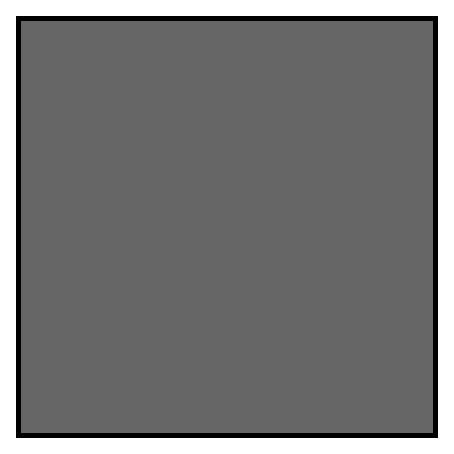
\includegraphics{example.eps}
% figure caption is below the figure
\caption{Please write your figure caption here}
\label{fig:1}       % Give a unique label
\end{figure}
%
% For two-column wide figures use
\begin{figure*}
% Use the relevant command to insert your figure file.
% For example, with the graphicx package use
  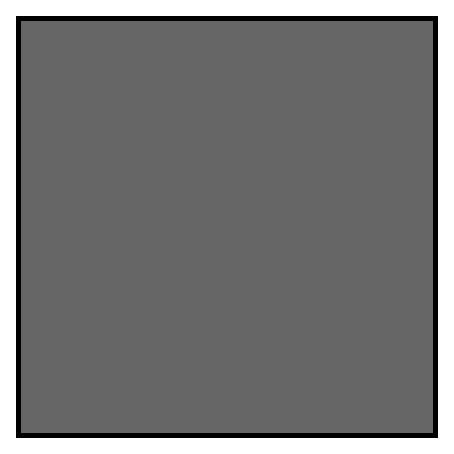
\includegraphics[width=0.75\textwidth]{example.eps}
% figure caption is below the figure
\caption{Please write your figure caption here}
\label{fig:2}       % Give a unique label
\end{figure*}
%
% For tables use
\begin{table}
% table caption is above the table
\caption{Please write your table caption here}
\label{tab:1}       % Give a unique label
% For LaTeX tables use
\begin{tabular}{lll}
\hline\noalign{\smallskip}
first & second & third  \\
\noalign{\smallskip}\hline\noalign{\smallskip}
number & number & number \\
number & number & number \\
\noalign{\smallskip}\hline
\end{tabular}
\end{table}


%\begin{acknowledgements}
%If you'd like to thank anyone, place your comments here
%and remove the percent signs.
%\end{acknowledgements}

% BibTeX users please use one of
%\bibliographystyle{spbasic}      % basic style, author-year citations
%\bibliographystyle{spmpsci}      % mathematics and physical sciences
%\bibliographystyle{spphys}       % APS-like style for physics
%\bibliography{}   % name your BibTeX data base

% Non-BibTeX users please use
\begin{thebibliography}{}
%
% and use \bibitem to create references. Consult the Instructions
% for authors for reference list style.
%
\bibitem{RefJ}
% Format for Journal Reference
Author, Article title, Journal, Volume, page numbers (year)
% Format for books
\bibitem{RefB}
Author, Book title, page numbers. Publisher, place (year)
% etc
\end{thebibliography}

\end{document}
% end of file template.tex

